\chapter{\label{controlled-rotations}Controlled Rotations}

\section{Singly-Controlled Rotations}
Singly-controlled Z rotation.

\begin{figure}[hb]
    \centering
    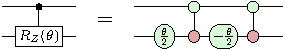
\includegraphics[width=\textwidth]{controlled-rotations/CRZ}
    % \caption{}
    % \label{}
\end{figure}

Singly-controlled X and Y rotations obtained by conjugating the control qubit.

\begin{figure}[hb]
    \centering
    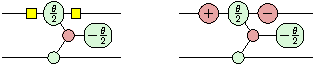
\includegraphics[width=0.6\textwidth]{controlled-rotations/CRX_CRY}
    % \caption{}
    % \label{}
\end{figure}

\section{Doubly-Controlled Rotations}
hello world


\section{Triply-Controlled Rotations}
hello world
hello world
